\chapter{Learning and creativity in organisations} \label{learning}
\textit{"The organisations that will truly excel in the future will be the organisations that discover how to tap people's commitment and capacity to learn at all levels in an organisation."} \citep{senge1990fifth} 
\newline
\newline
Everyday problem-solving and immediate reactions to situations at hand are often related to performing instead of learning. Furthermore, long-term adaptations to our previous experiences and beliefs is mainly considered as developing, not learning. Yet, when talking about development and developing in individual, team or organisational level, the question highly concerns and is related to learning. \citep{kolb1984experiential}

In order to support growth and learning in organisational and business levels, the learning process needs to be understood all from organisational, team and individual perspective \citep{buijs2007innovation}. In this chapter, learning is first outlined in organisational level, following individual and team perspectives. Furthermore, concept of a learning organisation is presented and building blocks for it are presented. 

Uncertain and unpredictable problems and business requires creativity and innovation abilities of organisations and its employees. Thus, this chapter also describes aspects of creativity of an individual and outlines factors to support creativity of employees. 

This chapter forms the basis and background for the next chapter, which introduces experimentation-driven development process as a tool for innovation, developing and learning. 

\section{Organisational learning}
Generally organisations are considered as machines, yet recently more emphasis has been put on organisations as living organisms. When considered as a machine, organisational model is mechanic and simple, which purpose is to gain profit. Organisation as a living organism refers to a whole-systemic model, where employees find meaning in their work and are able to grow. Liable vision of the future and this thesis focuses on the latter perspective of organisations, where learning and renewal form the essence of being. \citep{geus1997living}  Also according to \citet{edmondson1999psychological}, learning is an essential concern in the fast-paced working environment, where organisational change and complexity are increasing.  

Organisational learning is approached conventionally from two different perspectives in the literature. On the one hand, learning is considered as an outcome, and on the other it is considered as a process \citep{edmondson1999psychological}. In the first perspective organisational learning is referred to be \textit{"an outcome of a process of organisations encoding interferences from history into routines that guide behaviour"} \citep{levitt1988organizational}, whereas process perspective defines learning as a process of continuous trial and error \citep{argyris1978organizational}. In this thesis, learning is considered as the latter tradition of learning, which allows growth and improved performance of individuals and organisations.

Educational philosopher John Dewey has conceptualised learning as a process in his writings about inquiry and reflection \citep{dewey1956human}. His work has influenced remarkably on following learning theories, such as experiential learning theory \citep{kolb1984experiential} or action approach of organisational learning \citep{schon1983reflective}. According to \citet{dewey1956human} learning is an iterative process consisting of designing, carrying out, reflecting upon and modifying actions. Dewey separates learning from humans' tendency to behave habitually or automatically. \citet{edmondson1999psychological} builds to this definition focusing on the group level of learning and defining it as an ongoing process where reflection and action occur. Integral characteristics of learning process are asking questions, seeking for feedback, performing experiments and reflecting on the results, having discussions about errors and surprising or unexpected outcomes of actions.

According to \citet{march1991exploration} learning consists of exploitation, exploration and adaptation. Exploitation refers to refinement and extension of competences, technologies and paradigms that already exist, whereas exploration is about experimentation with new approaches and alternatives. When results and returns of exploitation are often positive, proximate and predictable, returns of exploration are uncertain, distant and usually negative. Therefore, exploration leads to greater locus in learning and realisation of problems than exploitation, when considered the distance in time and space. \citep{march1991exploration}

Accordingly, in management literature learning is considered relating and even being dependent on receiving feedback \citep{schon1983reflective}, discussion and failure \citep{sitkin1992learning} and experimenting \citep{henderson1990architectural}. As relevant information about performance is acquired through errors, discussion about them has been related with organisational effectiveness \citep{sitkin1992learning}. According to \citet{huy2003rhythm} organisations learn best through small experiments and trying out new things, and the closer and more related experimentations are to customers and customer interfaces, the more can be learned. 

Organisational learning research puts emphasis on cognitive and interpersonal variables when explaining effectiveness in teams and individuals, where it can also be also explained through organisation and team structures \citep{edmondson1999psychological}. For instance, \citet{argyris1993knowledge} has argued how individual's negative beliefs about communication and interaction may inhibit learning behaviour and lead to ineffective working in an organisation. 

According to \citet{march1991exploration} learning is a significant factor in improving organisational performance and strengthening competitive advantage. Accordingly, it is the essence of developing and innovation; \citet{buijs2007innovation} even claims all innovation processes are processes for organisational learning. Also \citep{quinn1985managing} argues how especially from the management perspective major innovations should be considered as incremental and interactive learning processes driven by certain goal.  

\section{Experiential learning on individual level} \label{individual}
Various perspectives and definitions for learning has been studied, presented, analysed and utilised in order to understand individual's process of adapting new information and skills. Experiential learning theory refers to learning as a process of knowledge-creation through experiences while experiential learning process stands as a way to describe the central process of human adaptation to the social and physical environment - a holistic adaptation process that provides bridges across life situations and acts as a base for the lifelong process of learning. \citep{kolb1984experiential}. Also \citet{jung1923psychological} argues how learning involves concept of human being as a whole - from feeling and thinking to perceiving and behaving.

Experiential learning theory of \citet{kolb1984experiential} consists of four elements: experience, perception, cognition and behaviour. Immediate experience forms a basis for reflection and observation, following assimilation to a theory from which new implications for action are deducted. In order to create new experiences, these implications serve as guides. Overall, experience of an individual is a focal point of learning giving personal meaning to abstract concepts, which can be afterwards shared with others. Furthermore, receiving feedback serves a continuous process for goal-oriented action following evaluation of that action. Feedback can thus boost effective, goal-oriented learning process. \citep{kolb1984experiential}

Continuing with the model of \citet{kolb1984experiential}, instead of conceiving learning in terms of outcomes, it should rather be conceived as a process. Ideas are not fixed and and immutable elements of thoughts, but can be formed and re-formed through experience. Furthermore, bringing the experiential learning into educational implications, all learning can be considered as relearning. Thus, all learning situations should take into account people arriving from all different experiential backgrounds to what they build their new experiences and knowledge on. This partly explains resistance to new ideas, as when new information and experiences are in contradiction to old beliefs and experiences, new ideas and information is more difficult to adapt. In the education process learner's old beliefs and theories should be brought out, examined and tested, following integration of the new models and refined ideas into learner's belief systems. \citep{kolb1984experiential}

\citet{kolb1984experiential} presents Piaget's interactive process approach to learning, according to which individual learning and adaptation of new ideas occurs through integration or substitution. Integration leads to stronger part of learner's conception of the world, whereas substitution requires real questioning of previous conceptions, and thus might take longer for the learner to adopt. Learning is a mutual process between accommodation of concepts or schemas to experiences around us and assimilation of events and experiences into existing concepts and schemas. This intelligent adaptation, learning, results from the tension between accommodation and assimilation. Through this tension growth and higher-level cognitive functioning occurs.\citep{kolb1984experiential}

According to \citet{kolb1984experiential}, learning is a process filled with tension and conflict, and new knowledge, skills and attitudes are achieved through experiential learning, which consists of four modes and required abilities of learners: concrete experience abilities, reflective observation abilities, abstract conceptualisation abilities and active experimentation. Individuals must openly involve themselves in new experiences, reflect and observe them from various perspectives, create concepts that can be integrated into more abstract theories as well as they need to be able to use these reflections and theories in active daily decision-making and problem-solving.  

\section{Team learning and performance} \label{teamperformance}
According to \citet{hammer1993reengineering} role of employees is changing to more autonomous performing multi-dimensional knowledge work rather than simple and detailed tasks under strict control, and organisational structure is changing from functional departments into process teams. This together with fast-pace environment requires organisations to enhance the ability of teams to learn and create safe environment for learning. Thus, pressure on managers to understand and enhance team efficiency, work and learning has increased. \citep{edmondson1999psychological}

Work team refers to small group of people that exist within the context of a larger organisation, members share understanding of being a member of the team and its tasks, responsibility for a product or a service a team is working on \citep{hackman1987design,alderfer1983intergroup} as well as its performance \citep{edmondson1999psychological}. Additionally, team members have supplementary knowledge and abilities compared to each other, and they share a goal, targets and ways of working and approach \citep{edmondson1999psychological}. According to \citet{katzenbach1993wisdom} great team performance consists of continuous work of shaping a common purpose, agreeing on performance goals, defining a common working approach, developing high level complementary skills and being transparent on the results. He emphasises that through disciplined actions groups transform to teams and argues how demanding schedules, long-standing habits and unwarranted assumptions tend to threaten team efficiency and performance\citep{katzenbach1993wisdom}. In group level, learning is enabled through testing assumptions and discussion of opinion differences transparently in order to improve team performance\citep{edmondson1999psychological}.

Indeed, learning behaviour of teams refers to activities that team members carry out and through which team is able to obtain, adapt and reflect data and outcomes of actions which further shapes and improves team behaviour. Such activities consist of reflection and improvement-aiming factors including asking for feedback, transparent information sharing, asking for help, admitting and discussing about failures and errors as well as experimenting. Through such activities teams may observe changes in environment, customer requirements and improve collective understanding. In addition, team's ability to discover and react to unexpected situations and consequences of their actions is likely to improve through learning behaviour. Consequently, compared to low-learning teams that tend to get stuck and are unable to solve problems, teams who master in learning are greater in confronting difficult situation and improve their work. \citep{edmondson1999psychological}

\citet{edmondson1999psychological} have studied factors that affect and influence learning behaviour in teams by studying in which conditions and to what extent learning occurs naturally. Based on her research, \citet{edmondson1999psychological} created a concept of psychological safety, which refers to team's confidence, shared belief and mutual trust among team members towards that speaking up in a team does not lead to embarrassment, rejection or punishment of any kind \citep{edmondson1999psychological}. This concept has roots already in early research on organisational change. \citet{schein1965personal} state that in order individuals to change and feel safe they need psychologically secure environment. However, team psychological safety should not be confused with groupthink effect that refers more to group cohesiveness, which seems to be related to decreased willingness to disagree and challenge team member's views and thus reduces interpersonal risk-taking \citep{janis1982groupthink}.

\section{Learning organisations and its building blocks}
 \textit{"Learning organisation is an organisation, where people are able to constantly develop and achieve intended results; where new ways of thinking are born and where people share goals and learn together."} \citep{senge1990fifth}
\newline

The description above for learning organisation from \citet{senge1990fifth} is one of the most famous. According to \citet{garvin2008yours} in learning organisation employees excel at creating, acquiring and transferring knowledge. In order to improve long-term learning of an organisation, strengths and weaknesses of an organisation and its unit needs to be recognised. They also define three building blocks to support learning organisation, which are supporting learning environment, concrete learning processes and practices and leadership behaviour that reinforces learning. These building blocks can be considered and measured as independent components yet each of them vital to the whole, as learning is a multidimensional phenomenon. \citep{garvin2008yours} 

 \citet{edmondson1999psychological} presents and studies behaviours through which various outcomes of learning as adaptation to change, understanding or improved performance are likely to be achieved. Supporting learning environment refers much the same concept as psychological safety of  \citet{edmondson1999psychological} described in section \ref{teamperformance}. According to \citet{edmondson1999psychological} team psychological safety should be the first essential building block of learning behaviour in work teams. Supporting learning environment consists of four characteristics: psychological safety, appreciation of differences, openness to new ideas and time for reflection \citep{garvin2008yours}.

Concrete learning processes and practices includes experimentation, information collection, analysis, education, training and information transfer. Learning organisations can be supported through concrete steps and activities which are tested and further developed through experimentations. Furthermore, information and intelligence about customers as well as technological trends should be collected systematically and further analysed focusing on identifying problems and solving them. Training and education of new and established employees is an essential part of practices and processes. Finally, through transparent and meaningful knowledge sharing organisational learning can be enhanced, focus being on clear, well-defined and working communication systems that employees can easily relate to. Concrete processes together with efficient knowledge sharing methods ensure essential information being available fast and efficiently for employees to use. \citep{garvin2008yours}

Leadership behaviour should reinforce learning. This requires new way of leadership \citep{shalley2004leaders}: instead of leading the work, role of the leaders is turning to more coaching-oriented \citep{hammer1993reengineering}. Behaviour of leaders is highly related to the performance of employees \citep{kim2014blue} and organisational learning \citep{garvin2008yours}. In order to encourage learning of employees, leaders should prompt dialogue and debate, ask questions and listen to employees \citep{kim2014blue,garvin2008yours}. Yet, supportive leadership behaviour alone is not sufficient guarantee for organisational learning. \citet{garvin2008yours}emphasise how organisations are not monolithic and managers should sense differences in culture, department and units. In addition to cultural differences, learning requires clear and targeted processes and practices. 

Leadership behaviour helps in creating supporting learning environment, which supports managers and employees in creating and defining concrete learning processes and practices. Furthermore, concrete processes support leaders' behaviour in a way that fosters learning and through own example cultivates that behaviour to others. \citep{garvin2008yours}

\section{Creative individual}
Divergent thinking refers to an individual's ability to find multiple alternative solutions and ideas to problems, and has been related to serve as a key capacity affecting creative thinking \citep{guilford1967creativity}. \citet{amabile1996assessing} defines creative thinking as a way how people approach problems and come up with solutions. Thus, creative thinking refers to a combination of past experiences creating expertise and the ability to apply creative thinking skills to these experiences and invent new solutions. \citep{amabile1998kill}

Recently problem construction processes have been recognised and combined to everyday problem-solving and real-world creativity \citep{getzels1975problem,runco1988problem}. According to study of \citep{gardner1988creativity} correlation between creative problem solving and everyday problem solving exists: they seem to have the same roots in information processing skills. Indeed, problem finding and construction, making connections and evaluating ideas are important for creativity \citep{mumford2002leading,vincent2002divergent}. Thus, when improving individual's possibilities to multiple alternatives, related ideas and example solutions, they tend to make more connections leading to creative actions \citep{amabile1996assessing}. 

Accordingly \citet{mumford1988creativity} emphasis that creative people consistently and with confident tend to seek for alternative solutions, even under uncertain conditions. Even though expertise and intelligence have been related to problem solving, series of causal analyses carried out by \citet{vincent2002divergent} revealed unique effects divergent thinking had that were not attributed to intelligence and expertise. 

Several factors form the basis of creativity skills of an individual, essential being personality and personal characteristics \citep{mumford1988creativity,jung2003role,redmond1993putting}. Studies show employees who consider and believe creativity as valued outcome and believe in their own creative abilities are more willing to generate ideas, experiment, communicate openly with others about ideas and through this, overall, their behaviour will eventually lead to creative outcomes \citep{shalley2004leaders}. Accordingly, \citet{csikszentmihalyi199916} presents the belief and feeling an employee has on the capabilities, pressure, resources and socio-technical system of work environment affects highly on the success of creativity. 

Intrinsic motivation is claimed to be one of the most powerful tools to creative action and non-traditional thinking \citep{amabile1996assessing,deciintrinsic,jung2001transformational}, as intrinsically motivated individuals usually prefer novel solutions, challenging status quo and trying out new ways for problem-solving \citep{amabile2002creativity}. Broad interest stands as a sign of intrinsic motivation, which is also widely related to both creativity and well-being of an individual and innovation (e.g. \citep{hennessey19881,csikszentmihalyi199916,gardner1988creativity,shalley2004leaders}). In their study  \citet{tierney1999examination}, found positive correlation between employee's level of enjoyment while working on a creative task at hand and the level of creativity. The study of \citet{redmond1993putting} showed how through motivational mechanisms, such as self-set goals, involvement and commitment, problem construction may have positive influence on solution quality and originality. Thus, problem construction is likely to have its greatest impacts on performance when in the process employee is allowed to express his values, needs and interests\citep{redmond1993putting}. Accordingly, \citet{shalley2004leaders} relate this to autonomy and independence in decision-making of an individual  

Meaning of prior knowledge and experience of an employee of area of work before demanding or anticipating creative actions from them is related to creativity \citep{mumford1988creativity,redmond1993putting,shalley2004leaders}. According to \citet{mumford1988creativity} and \citet{redmond1993putting} without previous experience of the job routine and substance knowledge and expertise on the field creative endeavours are more rare. Also \citet{jung2003role} argues for technical knowledge of an individual for fostering creativity. However, even though has been argued how routine work and task familiarity is likely to lead to habitual performance \citep{ford1996theory}, knowing the status quo may provide opportunities for creative actions and solutions through reflecting and practising skills required in the field. \citep{shalley2004leaders,andriopoulos2000enhancing} Although job rotation and employees from different areas works as a great source for new perspectives and development, creativity requires sufficient level of familiarity of target area \citep{shalley2004leaders}.

\citet{shalley2004leaders} argue that through developing extensive set of skills, employees may learn to be more comfortable and confident in thinking from different perspectives, finding various alternative solutions, trying out novel things and seizing opportunities. Individual creativity requires ability to work in a team, communicate, learn and reflect own learning \citep{roffe1999innovation} to receive feedback \citep{jung2003role}, ability to generate alternatives, engage in divergent thinking and tolerate or suspend judgement \citep{hennessey19881} .Through this perspective creativity can be considered as a skill that can be learned and strengthened. 

\section{Supporting creativity in organisations}
\citet{oldham1996employee} consider creativity skills and characteristics of and individual important, yet they add the importance of characteristics of organisational context such as job complexity, supporting supervision or controlling supervision. According to \citet{roffe1999innovation} creativity and innovation in an organisation require integrated organisational approach, right climate, appropriate incentives for innovators, and a systematic way and resources to transform an idea into an innovation. In addition,\citet{jung2003role} refers to strategy, structure, culture and available resources being essential in organisational level whereas in group level creativity skills consist of task structure, communication styles and task autonomy. 

\citet{amabile1998kill} has identified three factors being important for stimulating creative behaviour in individuals and organisations: individuals' intellectual capacity (creative thinking skills), expertise based on past experience and supporting work environment for creativity.  In addition, needs to be noted and understood that employees' thinking styles are shaped through what is rewarded, meaning that if organisational environment rewards well-behaving and instruction-following thinking style and action, employees tend to implement their style to that. We are urged to adapt to organisational style and fit in, and when this is not possible, people tend to leave. \citep{sternberg1997creativity}

Creativity is not restricted to artistic occupations only; it is required in various professions in which work tasks involve complex, ill-designed problems where novel solutions are needed and status quo challenged \citep{mumford1988creativity}. Indeed, idea implementation may require even more creativity than idea generation \citep{mumford2002leading}. In addition, depending on the job, different level and amount of creativity is required. Certain jobs that are highly involved with novel solutions urges for creativity as major breakthrough and innovative ideas, whereas more routine and repetitive jobs such as assembly line work requires creativity in developing the job practicalities. \citep{shalley2004leaders} 

Even though not all jobs require same amount of creativity, all organisations benefit from understanding where creativity is required and how it can be fostered and managed \citep{shalley2004leaders}. Likewise, creative actions of an employee are not worthwhile for an organisation when not coordinated or harnessed to yield organisational-level outcomes \citep{jung2003role}. Thus, the future focus should be in organisations' ability to mobilise creative actions of employees to create novel, socially valued products or services and more efficient ways of working \citep{mumford1988creativity}. 

Creative work is resource intensive where risk is involved \citep{mumford2002leading}. It is demanding and time-consuming \citep{mumford2002leading} and requires attention over long periods of time involving high level of ambiguity and stress \citep{kasof1997creativity}. Thus, organisational environment plays a major role in supporting employees' creative skills, and such stifling factors include for instance positive challenge at work, encouragement from organisational level, support from work group as well as supervisory encouragement. Furthermore, organisational impediments can lead to decreased level of creativity. \citep{amabile1998kill} 

Generation of novel, alternative solutions requires problem-finding skills \citep{runco1988problem}, which has been indicated to be one of the best predictors of creativity in 'real world' activities, when studied 91 elementary school students \citep{runco1990evaluating}. These findings suggest leaders, in order to enhance creativity of employees, to support learning of these skills for instance by facilitating problem-construction \citep{redmond1993putting}. In their study \citet{redmond1993putting} found leaders who supported employees problem-finding and problem construction skills and encouraged in generating multiple alternatives lead to more unique and novel solutions. 

According to \citet{isaksen1983toward} in order to support employee's creativity, leaders should focus on creating and maintaining an environment of supportive empathy, respect, warmth, concreteness, genuineness, trust and flexibility. These factors have been combined to general and task-specific efficacy needs \citep{mumford1988creativity}. Furthermore, through providing enough processing time for creating novel solutions is likely to enhance creative behaviour of employees \citep{isaksen1983toward}. As creativity refers to finding novel solutions and generating understanding of problems at hand, leaders could facilitate the process of resource allocation, feedback and task management \citep{mumford1988creativity}. In order to achieve novel solutions and fresh ideas, leaders may seek employees who have great knowledge and expertise or provide employees education and possibilities to develop their problem construction skills and furthermore encourage approaching problems from various perspectives. \citep{redmond1993putting} Overall, instead of managing creativity leaders should manage for creativity \citep{amabile2008creativity}.

Furthermore, pre-set obstacle, such as a deadline, assists in focusing individual's attention to an urgent problem, and has been noticed to stimulate creativity \citep{andriopoulos2000enhancing}. As employee who has the feeling of autonomy performs better, setting a deadline is not likely to threaten that autonomy, whereas showing someone how to meet that deadline would do \citep{mumford2002leading}. In addition, supporting employee's feeling of self-efficacy is likely to improve creative skills of an employee \citep{redmond1993putting}, and can be done through giving positive and realistic feedback, allowing adequate resources and physical support, clarifying task assignments, providing development support for employees, and assigning employees to appropriate tasks \citep{hennessey19881}.

Where leaders have a great role in enabling creative behaviour in teams and individuals, team members also influence essentially in others. Thus, by utilising various human resource practices leaders should create an environment where creativity is encouraged and supported. \citep{shalley2004leaders} Study of \citet{ancona1992demography} argue how changing the structure of teams may not be sufficient and does not lead to improved performance. Rather the leader and the team should find ways to foster positive effects of the team processes and reduce the negative ones. At team level this may mean focus on enhancing negotiation, problem-solving and conflict resolution skills while at organisational level leader should protect the team from external political pressures and reward the team from performance outcome instead of functional ones. \citep{ancona1992demography}

\section{Summary}
In this chapter learning was approached from organisational and individual perspective, supported by team perspective and performance in an organisation. Learning was defined as experiential-based iterative, life-long process of an individual and definition of learning organisation consisting of people developing and achieving intended results, aiming for novel ways of thinking, thriving for shared goals and learning together \citep{senge1990fifth}. Conditions enabling learning organisation were defined to be supporting learning environment, concrete learning processes and practices and leadership behaviour that reinforces learning. 

In addition, need for creativity in organisational and individual level was described and ways to support creativity and creative actions in organisations were introduced. 

Attributes provided in this chapter are essential to understand when considering novel approaches for development and new-value creation. Next chapter will present an experimentation-driven approach to developing as an alternative for conventional, planning-based developing. 
 
\chapter{Experimentation-driven development} \label{expe}
\textit{"What I hear I forget. What I see I remember. What I do I understand."} Lao Tse, Chinese philosopher
\newline

In the introduction part change in organisational and business environment were presented, forming background for the need of new methods to deal with change. This chapter presents experimentation-driven approach as such a method for developing and learning. 

Even though innovation and innovation processes were not in the focus of the study, experimentation serves as a method to foster innovation and is mostly brought up to the academia through innovation literature. Thus, it is an essential approach to contemplate together with the topic of experimentation. In the first section of this chapter, innovation process is briefly presented. 

This chapter outlines the relation between experimenting and innovation, describes the experimentation-driven process for development, serves examples on experimentation in action and outlines how experimenting can be considered as a method for learning. 

\section{Innovation process}
According to \citet{buijs2007innovation}, innovation consists of coming up with novel ideas and implementing them. Also \citet{vincent2002divergent} argues whereas creative processes comprise of initial idea generation, innovation process goes beyond the activities underlying the implementation of those ideas. 

Innovation process is a series of stages for processing the idea, and in the end of every stage the idea is reflected and evaluated before further processing. Evaluation points stands for usable tool for measuring the quality of idea but gives also understanding of how the evaluation process is going. In addition, while evaluating, team members also need to reflect the process and the idea, through which learning occurs. \citep{buijs2007innovation} Several other studies confirm how only after evaluation of ideas implementation should be discussed and performed \citep{mumford2002leading,vincent2002divergent,runco1994problem}. Useful questions in evaluation process could be "What went well?", "What can be improved?" and "What has been learned?" \citep{buijs2007innovation}. 

According to \citet{buijs2007innovation} innovation process itself can be approached from several angles: first of all, content of the innovation has to be clear - whether the purpose is to innovate new products, manufacturing processes, ways of organising work or ways of dealing with people. Secondly, psychological process of the innovation team has to be understood, essential being shared understanding, level of comfort with ambiguity and degree of trust between team members. Thirdly, creative process of the team, referring to idea generation processes, needs to be understood and efficiently facilitated. (ibid) \citet{amabile1996assessing} list similar attributes to contribute innovation: idea generation, creating climate of autonomy, engaging employees in their work and rewarding with both intrinsic and extrinsic rewards. 

\section{Experimentation in innovation processes} \label{expeinnovation}
When dealing in unpredictable, complex and uncertain environments, traditional ways for developing and innovation are not efficient, tend to take lot of resources and are too specification-driven, where specifications of the product or serviced are locked in the beginning of the project. In recent years the centre of innovation discussion in management and business literature have shed light on the concept of early, rough and iterative experimentation process models on innovation \citep{thomke1998managing,tuulenmaki2011art}.

\citet{thomke1998managing} defines experimentation as an essential part of innovation activity, relating it to the innovation process as a whole that has effects on the cost and time of the process. \citet{mumford2002social} argues in his study of Ben Franklin's social innovations, that the key factor in successful social innovation lays in fast demonstrating, which he also refers as experimenting. Even though literature on innovation focuses on organisational-level structures and processes, the innovation process and organisation's ability to launch a new product or service, create new value and processes as well as leverage novel technologies begins with individual employees presenting their ideas out loud and trying out novel approaches. \citep{argote2000knowledge} Thus, forming understanding of conditions that foster experimentation behaviour of individuals is important in order to support organisational innovation \citep{thomke2003r}. 

In this thesis experimentation refers to a personal trial and error process in which employees utilise their full potential \citep{andriopoulos2000enhancing}. Experimenting serves as a method for testing and validating abstract concepts \citep{kolb1984experiential} and dealing with novel products, ideas and processes. Innovation literature describes experimenting essential for new value-creation. Through experimenting essential factors concerning the final product are revealed before resources are overly spent, and through small failures success can be reached both earlier and faster. \citep{thomke2003r}

Experimenting as a means to develop and foster innovation is not a new approach. Discoveries such as artificial vaccines, flying and electric light bulb were results from iterative, trial-and-error process where knowledge was created trough iterations. \citep{thomke2003r} For instance, development process that lead to the innovation of a light-bulb consisted of repeated iteration of experiments, analysing the outcomes, learning from them and making changes for the next experiment. \citep{thomke2001enlightened} In addition, the significance and benefits of early experimenting or prototyping have been long recognised in working fields featuring complexity and unclarity, such as industrial and interaction design \citep{blomkvist2011conceptualising}. 

According to \citet{thomke2001enlightened}, in the beginning of every product is an idea, that was being shaped through the process of experimentation, and the ability to conduct experiments is actually a measurement of company's ability to innovate. 

According to \citet{quinn1985managing}, fast multiple-idea prototyping leads to more innovative outcomes, offers essential information about ideas or product's quality, motivates employees, and helps the company and the team to cope with anxiety and uncertainty in development. Thus, fast prototyping serves an essential way for learning from the iterative process. Market analysis, however, remain valuable when dealing with familiar products, yet with radical innovations they may easily offer misleading information. \citep{quinn1985managing}

Bank of America has conducted experiments several years in order to create novel service concepts for retail banking. They have set up an experimentation laboratory in some of their banks where customers during normal office hours can test novel ideas. Feedback is collected and experiments measured in order to learn for further experiments. During this process Bank of America has learnt radically about the system approach and deepened their understanding of the dynamics of service innovation. They have gained valuable insights and competitive advantage. \citep{thomke2003r}

Experimentation-driven approach for innovation differs from other methods for managing uncertain and innovation-focused projects in that it emphasises learning more than other methods. Overall, experimentation serves as a tool and everyday practice to guide company's strategy-making, business models and behaviour \citep{davenport2009design,mcgrath2010business}.

\section{Process for experimentation}
In the heart of problem-solving process is continuous trial and error which are directed by some amount of insight about the possible direction of the solution \citep{baron2000thinking}. Experimentation refers this iterative trial-and-error process where every trial provides new information of a problem \citep{thomke1998modes}. Through each trial new information is generated that would be challenging or even impossible to know in advance. Subsequent experiments are modified based on the information learned from previous trials, and in many cases this affects the way experiments are designed, conditions they are conducted in or even changes the direction of the desired solution. \citep{thomke1998modes} Thus, supporting tasks for experimentation are those allowing multiple problem-solving trials as well as present opportunities to be used together with earlier knowledge enhancing overall learning. \citep{lee2004mixed}

Experimentation process is presented as an iterative four-step learning cycle presented in figure \ref{pic:process} consisting of setting a hypothesis, planning an experiment, executing it and analysing the results. In the first phase, experimentation is designed based on the previous experience or good guess on solution, so hypothesis is set. In second phase the experiment is planned and the needed prototypes or spaces are build for experiment, following third phase where experimentation is executed. Analysing phase is essential in order to learn from the results and process and being able to conduct the cycle effectively again. \citep{thomke1998managing} Through experimentation the fundamental assumptions behind an idea can be tested \citep{tuulenmaki2011art}.

\begin{figure}[ht]
  \begin{center}
        \subfigure{
           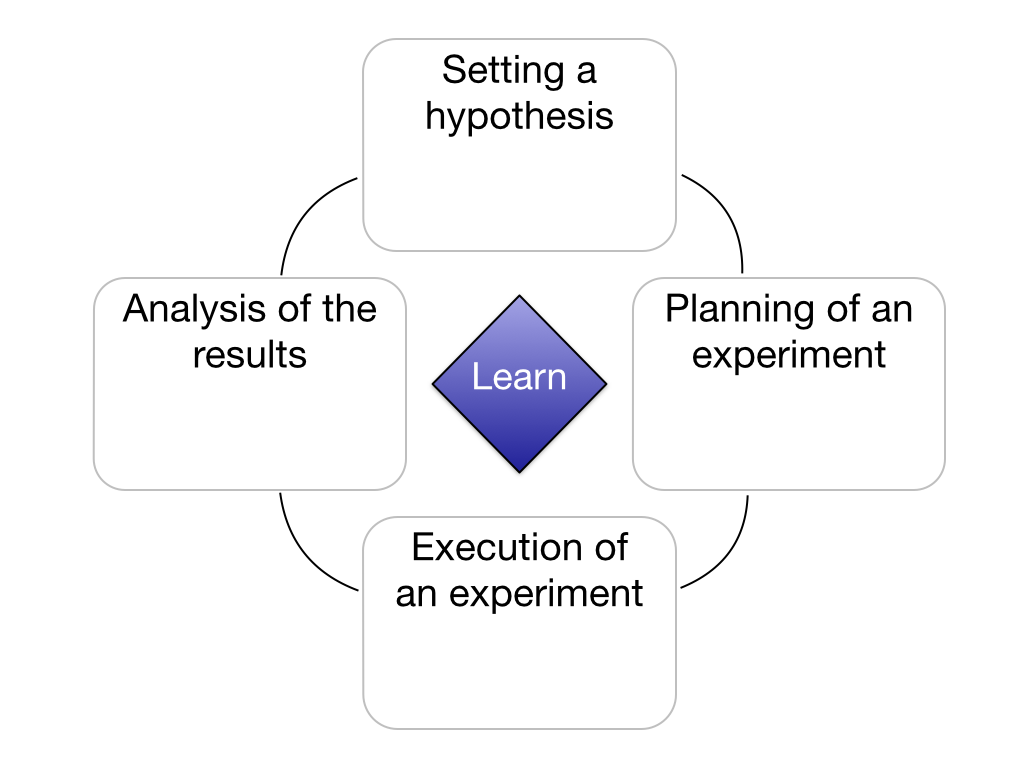
\includegraphics[width=0.83\textwidth]{process4.png}
    }
    \caption{Iterative learning process for experimentation, adapted from \citet{thomke1998managing}}
\label{pic:process}
   \end{center}
\end{figure}


%kuuluuko t�h�n? 
\citet{thomke2003r} defines several aspects to measure an experiment. These consist of fidelity, cost, iteration time, capacity, sequence, signal-to-noise ratio and type. Fidelity refers to an experiment conducted under conditions that represents actual use of final product, process or service in close detail. However, when testing in actual environment, various variables may affect on the experimentation setting, and this signal-to-noise ratio should be taken into account. Right balance between the speed of experimenting and receiving feedback in order to learn is crucial for successful experimenting, and this iteration time should be measured and estimated: time from the planning an experiment to the moment when results are available and further used. Also, cost of experiments should be analysed by estimating cost of designing, building, running and analysing experiments. Capacity concerns the realistic estimation of number of experiments possible to conduct with decent amount of fidelity in planned period of time. Experiments can be conducted in series or in parallel depending on the project at hand, and thus the sequence of experiments can be measured. Experiment type refers to the level of change, which can vary from incremental to radical. \citep{thomke2003r}

\subsection{Experimentation-driven models}
Conventional models for developing and innovating, such as stage-gate, consists mainly on planning the process and designing the solution without iterations. A pilot test is conducted in the very end of the process in order to finalise the project and solution. Commonly pilot tests consume significant amount of time and resources and end up in a notice that the product or service does not relate to customer needs. \citep{schrage1993culture}. Receiving feedback in this late phase of the project may lead to remarkable total costs and concurrently opportunities for innovation are lost. Experimentation-driven approaches focus on iterative testing and feedback loop, whereas conventional models emphasise the right solution with the first try. \citep{thomke2003r} Through experimentation new information and ideas can be generated and new opportunities can be found \citep{tuulenmaki2011art, mcgrath2010business}. 

Prototype-driven approach refers to a method in which customer feedback is acquired through prototyping in an early phase of the process in order to make changes in an affordable manner. Prototyping was noticed to be successful and lead to more successful products, produced with fewer design resources. Also higher customer satisfaction, quality and company's performance have been related to more flexible development process, in which changes can be made in the very late phase of the development process. \citep{thomke1998agile}

Experimentation is often conducted by using as simple prototypes of the intended-product as possible in order to experimentation remain light and cost-efficient. According to \citet{thomke2001enlightened}, critical part of innovation process occurs when first prototypes are generated, as at that point they can be further tested with customers, discussed and evaluated. However, experimenting only rarely leads to successful solution. Thus, planning and conducting multiple experiments in order to get closer to the problem solution is necessary. \citep{thomke1998modes} 

\citet{mcgrath2010business} offers an alternative model for experimentation-driven innovation, Discovery-driven Growth Process. In this model, instead of traditional yearly development of business, organisation sets an annual target and aims at experimenting it with as few resources as possible to learn from the target and clarify it the next year. In turn, the Lean Startup approach considers startup companies as a means of assuring and testing the strategy of an organisation to reveal which parts of it work and which do not work. \citep{ries2011lean}

According to Execution Innovation Model of \citet{tuulenmaki2011art}, experimentation-driven innovation process consists of series of iteration with the three idea types: opportunity idea, experimentation idea and execution idea. According to this model, new business can only be generated through a learning process of iterative experimentation, and specifications of the final business or product and final execution idea are decided only after several iterations that aim to validate and explore the implementation possibilities. \citep{tuulenmaki2011art} 

In this thesis, Execution Innovation Model is discussed in more detail. Figure \ref{pic:tuulenmakimodel} summarises differences between the execution innovation model and other development modes. 

An example to go through the phases of experimentation-driven innovation process is the story of Zappos, an online shoe retailer company, which at the moment is one of the most successful online shoe stores in the world. The owner of the company, Tony Hsieh, got \textit{an opportunity idea} to sell shoes online, without the need to go the store, all tired and frustrated. However, back in 2004 an idea of an online retailer for shoes was quite absurd, but Hsieh generated \textit{an experimentation idea} to test the hypothesis of people being interested in buying shoes online: he visited a local shoe store, asked permission to take pictures of a pair of shoes, downloaded the picture online and waited if potential customers found them and made a purchase. When this occurred, he returned to the store, bought the pair and shipped them to the first customer. Instead of writing a business plan a founder produced an experimentation idea: the easiest way possible to test whether the opportunity idea is worth further development. \citep{hsieh2010delivering} Through this experiment Hsieh learnt his idea was not all worthless and also gained major insights considering the whole process, and \textit{the execution idea}: purchasing, shipping, customer service, invoicing and customer wishes. From this small experiment Zappos has grown to one of the biggest online shoe retailer companies in the world \citep{hsieh2010delivering}. 

Opportunity idea refers to an idea which is imagined to solve specific problem and something that brings closer to the solution. Experimentation idea assists in testing the critical assumption and figuring out, whether the idea is worth taking further risks. Execution ideas are the outcomes from experimentation ideas, those ideas that have been through iterating and validating process chosen to further development and implementation. Execution ideas gather all the learnings from experiments, through which the original opportunity idea is modified in order to reach the final design plan. \citep{tuulenmaki2011art} 


\begin{figure}[!H]
\vspace{-300pt}
\hspace{-75pt}
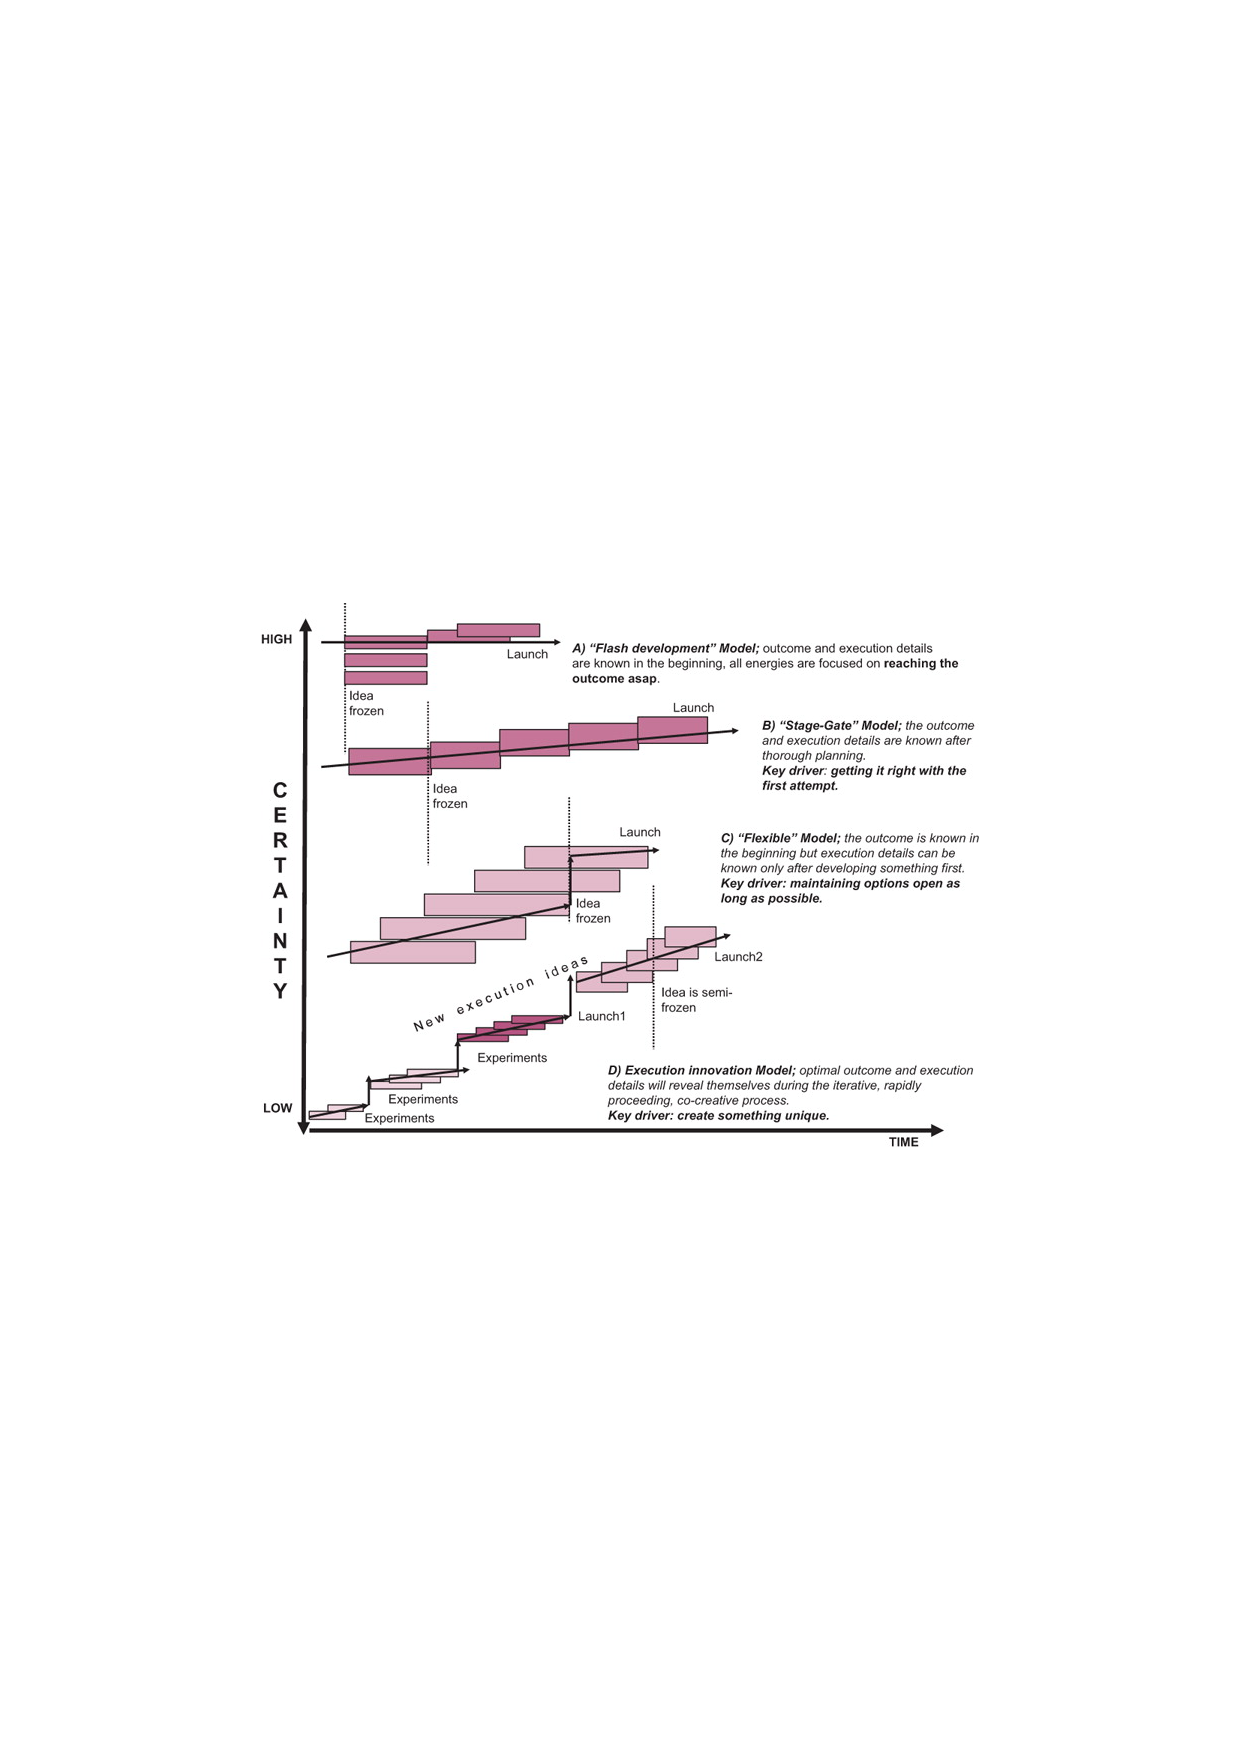
\includegraphics{tuulenmaki.pdf}
\vspace{-20pt}
\caption{Differences between the execution innovation model and other development modes \citep{tuulenmaki2011art}}
\label{pic:tuulenmakimodel}
\end{figure}


%

\section{Experimentation as a method for developing and learning}
According to \citet{edmondson1999psychological} and \citet{henderson1990architectural} experimenting and reflecting the results are essential characteristics of learning. \citet{march1991exploration} refers to exploration (experimenting with new approaches and alternatives) as a method to tolerate and learn from uncertain and distant outcomes. Also \citet{lee2004mixed} argues experimenting being fundamental for learning especially when dealing with problems with uncertain outcomes. Likewise, experimenting works when the most essential sources of information do not exist or are unreachable \citep{lee2004mixed}.

In addition, \citet{garvin2008yours} includes experimenting as an essential part for a learning organisation, experimenting serving as a tool for a concrete learning process and practice.  The amount and value of learning achieved from experiment defines its success: the more has been learnt and the more valuable insights, the more successful the experiment \citep{thomke2003r}. 

According to \citet{vincenti1990engineers} through experimenting new knowledge is created and engineer's understanding of new analytical concepts and ways of thinking widens. Accordingly, employees who improvise, practice their thinking and conduct experiments remain in the fierce competition of industries requiring constantly fresh ideas and innovations \citep{ciborra1996platform}.

The essence of learning from experiments is to figure out what works and what does not in an experiment or idea. Thus, experiments should be designed and planned keeping in mind how to maximise the amount of learning and valuable insights, not focus on wrong details and success of the experiment itself. Through defining accurate measures one can actually know whether the experimenta was useful and essential was learned \citep{thomke2003r}. 

\citet{thomke1998managing} defines experimentation efficiency, referring to "economic value of information learned during an experimental cycle, divided by the cost of conducting the cycle." The more inexpensive (costly) an experimentation is and the more valuable (valueless) gained information is, the higher (lower) is experimentation efficiency. 

Furthermore, experimentation is essential in order to learn about the idea, concept and prototype and whether it actually addresses a new need or a problem, or solves the one at hand \citep{thomke2001enlightened}. Prototyping is critical part of the process, as testing the prototype in a real environment gives instant and valuable feedback for further development \citep{thomke2001enlightened}. 

%kuuluuko t�h�n?
Anticipating and exploiting early information can save a lot of resources in the development process. According to IDEO, an innovation and design-firm, using human-centred design-based approach, the key elements in the design process and prototyping is it being rough, rapid and right. The right-element reminds that even though the prototype itself is likely to be incomplete, it has to show the right specific aspects of a product. This forces developers to decide the factors that can initially be rough and those that must be right. In addition, exploiting early information serves as a good method for developers reflecting changing customer preferences. Briefly, information in the early stage of the developing process should be listened and discovered carefully, as the problems are cheaper and easier to solve. \citep{thomke2001enlightened}

\section{Summary}
The aim of this chapter was to present experimentation-driven approach for developing. Through trial and error process various design alternatives can be tested and generated, essential being reflection after each experiment and making changes accordingly to next experimentation round.  \citep{thomke1998modes}

Experimenting stands as a method for learning: according to \citet{edmondson1999psychological} and \citet{henderson1990architectural} experimenting and reflecting the results are essential characteristics of learning, and \citet{march1991exploration} refers to exploration (experimenting with new approaches and alternatives) as a method to tolerate and learn from uncertain and distant outcomes. In addition, \citet{garvin2008yours} includes experimenting as essential part for learning organisation, experimenting serving as tool for concrete learning process and practice. 

Next chapter further describes factors essential for experimenting in organisational context. 